% Begin the document and set up the style of the document
\documentclass[a4paper]{article}

% Install the required packages for the document 
\usepackage{envmath}
\usepackage{esvect}
\usepackage{graphicx}
\usepackage{gensymb}
\usepackage{tikz}
\usepackage{geometry}
\usepackage{enumitem}
\usepackage{mathtools}
\usepackage{graphicx}
\usepackage{amsmath}
\usepackage{amscd}
\usepackage{amssymb}
\usepackage{amsfonts}
\usepackage{pgf}
\usepackage{tikz}
\usepackage{mathrsfs}
\usepackage{asyalign}
\usepackage{physics}
\usepackage{cite}
\usepackage{url}
\usepackage[tableposition=top]{caption}
\usepackage{ifthen}
\usepackage[utf8]{inputenc}
\usetikzlibrary{arrows}

\begin{document}

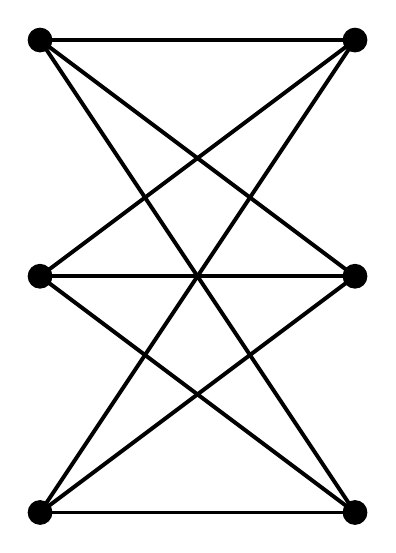
\begin{tikzpicture}

	\draw[line width = 0.5mm] (-2,-3) -- (2,3);
	\draw[line width = 0.5mm] (-2,3) -- (2,-3);
	\draw[line width = 0.5mm] (-2,3) -- (2,3);
	\draw[line width = 0.5mm] (-2,-3) -- (2,-3);
	\draw[line width = 0.5mm] (-2,0) -- (2,0);
	\draw[line width = 0.5mm] (-2,-3) -- (2,0);
	\draw[line width = 0.5mm] (-2,3) -- (2,0);
	\draw[line width = 0.5mm] (2,3) -- (-2,0);
	\draw[line width = 0.5mm] (2,-3) -- (-2,0);
	\draw[fill] (-2,3) circle (1.5mm);
	\draw[fill] (2,3) circle (1.5mm);
	\draw[fill] (-2,0) circle (1.5mm);
	\draw[fill] (2,0) circle (1.5mm);
	\draw[fill] (-2,-3) circle (1.5mm);
	\draw[fill] (2,-3) circle (1.5mm);

\end{tikzpicture}










\end{document}